The following figures were obtained using the procedure described previously.

\begin{figure}[h!]
    \centering
    \begin{minipage}[t]{0.48\textwidth}
        \centering
        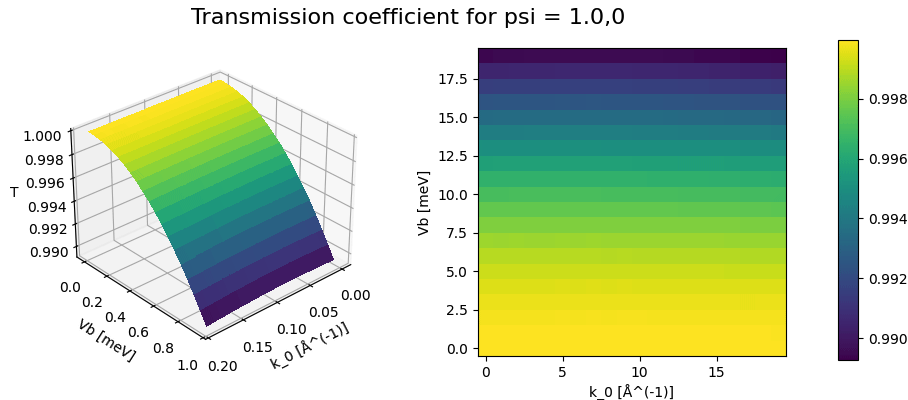
\includegraphics[width=\textwidth]{../assets/images/No-Rashba/TCoefficient(1.0,0)xalpha=0beta=0}
        \caption{figure}{
            Transmission coefficient ($T$) in pristine graphene with initial pseudospinor configuration $\xi = (1, 0)$, plotted against potential barrier height ($V_b$, in meV) and initial wave vector ($k_0$, in \AA$^{-1}$). The 3D plot and 2D heatmap show that transmission is largely independent of the initial wave vector but decreases noticeably as the barrier height increases, ranging from $1$ to approximately $0.990$.
        }
        \label{fig:noRashba}
    \end{minipage}
    \hfill
    \begin{minipage}[t]{0.48\textwidth}
        \centering
        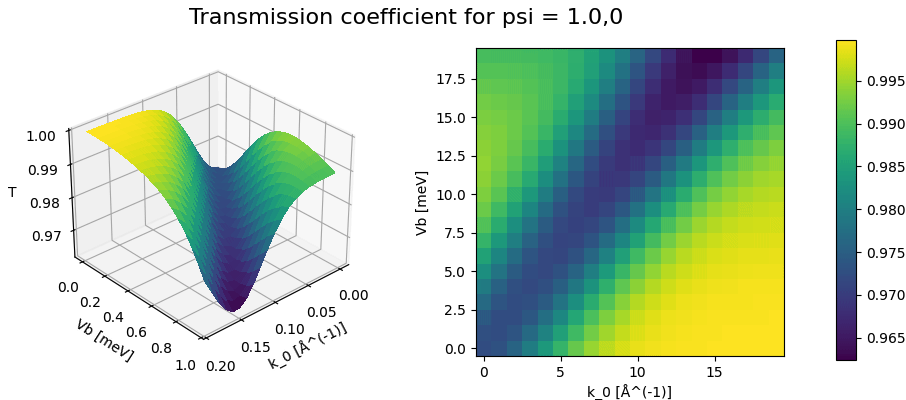
\includegraphics[width=\textwidth]{../assets/images/Rashba/TCoefficient(1.0,0)xalpha=0.2beta=-0.2}
        \caption{figure}{
            Transmission coefficient ($T$) as a function of potential barrier height ($V_b$) and initial wave number ($k_0$) with an initial pseudospinor configuration $\xi = (1, 0)$. The 3D surface and 2D color map show a non-monotonic dependence of $T$ with respect to $V_b$ and $k_0$, highlighting the influence of spin-orbit coupling on transmission through the barrier.
        }
        \label{fig:rashba}
    \end{minipage}
\end{figure}

In the images, we can observe certain interesting aspects, starting with fig.\ref{fig:noRashba}.
The image presents two graphs that illustrate the transmission coefficient ($T$) as a function of $Vb$ (in meV) and $k_0$ (in \AA$^{-1}$) for a fixed value of $\xi = (1, 0)$.
The left graph is a three-dimensional visualization where $T$ is on the $z$-axis, $Vb$ on the $x$-axis, and $k_0$ on the $y$-axis, with a color scale that varies from dark purple (lower $T$) to bright yellow (higher $T$).
The right graph is a two-dimensional heat map that offers a top view, with the $x$-axis representing $k_0$ and the $y$-axis representing $Vb$, using the same color map as the 3D graph.
Both graphs show that the transmission coefficient generally remains very close to 1, indicating high transmission.
As $Vb$ increases, $T$ tends to decrease, while the dependence on $k_0$ is minimal.
In general, the graphs demonstrate how $T$ changes with variations in $Vb$ and $k_0$, highlighting a slight decrease in $T$ as $Vb$ increases and an insignificant change with respect to $k_0$.

This result shows a contradiction with what is already specified in the literature, as in graphene, total transmission would be expected due to the material's inherent properties\cite{horsell2008, Young2009}.

These observed differences can be primarily attributed to the following aspects related to our method and simulation conditions:

\begin{itemize}
    \item Wave Packet Characteristics:
    Our simulation uses a wave packet (GWP) composed of multiple momentum eigenstates instead of considering a single eigenstate.
    This choice implies simultaneous contributions from several states, potentially generating quantum interferences that slightly affect the transmission coefficient\cite{Staelens2021}.
    This point, highlighted by our time-dynamic modeling, marks a significant difference compared to ideal theoretical models where such interferences do not appear.

    Additionally, our simulation explicitly considers the time variable, something uncommon in previous ideal and static theoretical studies.
    Investigating how these dynamic aspects, such as phase time or tunneling time, specifically affect the observed transmission is an important objective proposed for future work.

    \item Quantum interference effects due to packet dispersion over time:
    As suggested by the literature\cite{MolgadoMex2018}, when a sufficiently wide Gaussian wave packet evolves temporally, it disperses spatially in such a way that different parts of it simultaneously interact with the barrier, causing internal interferences with itself.
    Such interference is a possible additional cause of the fluctuations in transmission observed in our numerical results.
\end{itemize}

These points clearly explain the differences found from a methodological perspective and link our numerical results to the theoretical prediction mentioned in previous studies.
This not only clarifies the apparent contradiction but also clearly reinforces the connection between our specific results and the main objective of analyzing dynamic effects and properties that arise when using Gaussian wave packets in quantum tunneling simulations in graphene-based systems.

On the other hand, we have the transmission under the presence of SOIR (Fig.\ref{fig:rashba}).

A correlation between the variables is observed: generally, with greater potential barrier height ($Vb$) and greater initial wave number ($k_0$), lower transmission is expected.
However, the spin-orbit interaction introduces more complex behavior.
As $k_0$ increases and $Vb$ decreases, the transmission approaches 1, indicating a higher probability of quantum tunneling due to SOIR\@.

Although the variation in the transmission coefficient is small (on the order of $10^{-2}$), it is significant and attributable to the SOIR interaction. The electrons, with their different pseudospin components, interact, and this interaction is affected by the initial wave number of the Gaussian wave packet (GWP), as observed in previous studies\cite{Serna2019}.
Therefore, SOIR modulates the interaction, which in turn causes the fluctuations observed in the transmission coefficient.

It is important to highlight here that the analytical derivation of the current vector (eq. \ref{eq:componentes}) has been crucial for interpreting the numerically obtained results.
In particular, this equation allows explicitly linking observed differences in transmission coefficients with pseudospinorial components and their cross-correlations due to the Rashba interaction.
Therefore, this result not only provides conceptual clarity but also lays the foundation for future theoretical and experimental research on advanced spintronic transport in graphene.

After thoroughly analyzing the numerical results and discussing the particular aspects observed in the electronic transmission coefficients with and without Rashba interaction, we can synthesize below the main conclusions reached in this work, highlighting their theoretical and technological implications, as well as the perspectives for future studies and applications.
